\RequirePackage{etoolbox}
\documentclass[a4paper,man,natbib,floatsintext]{apa6}

\usepackage[english]{babel}
\usepackage[T1]{fontenc}
\usepackage[utf8x]{inputenc}
\usepackage[T1]{fontenc}
\usepackage{amsmath}
\usepackage{graphicx}
\usepackage[colorinlistoftodos]{todonotes}
\usepackage{hyperref}
\usepackage{apacite}
\usepackage{verbatim}
\usepackage{csvsimple}
\usepackage{enumitem}
\usepackage{multirow,booktabs,setspace,caption,siunitx}
\usepackage{tikz}
\usepackage{siunitx}
\usepackage{pdfpages}
\usepackage{longtable}
\usepackage{etoolbox}
\usepackage{environ}

\newtoggle{bibdoi}
\newtoggle{biburl}
\makeatletter

\undef{\APACrefURL}
\undef{\endAPACrefURL}
\undef{\APACrefDOI}
\undef{\endAPACrefDOI}

\long\def\collect@url#1{\global\def\bib@url{#1}}
\long\def\collect@doi#1{\global\def\bib@doi{#1}}
\newenvironment{APACrefURL}{\global\toggletrue{biburl}\Collect@Body\collect@url}{\unskip\unskip}
\newenvironment{APACrefDOI}{\global\toggletrue{bibdoi}\Collect@Body\collect@doi}{}

\AtBeginEnvironment{thebibliography}{
 \pretocmd{\PrintBackRefs}{%
 \iftoggle{bibdoi}
  {\iftoggle{biburl}{\unskip\unskip doi:\bib@doi}{}}
  {\iftoggle{biburl}{access from \bib@url}{}}
 \togglefalse{bibdoi}\togglefalse{biburl}%
 }{}{}
}



\usepackage{tabularx} 
\usepackage{longtable}
\usepackage{threeparttablex}
\usepackage{booktabs}
\usepackage{rotating}
\usepackage{pdflscape} 
\usepackage[misc]{ifsym}
\usepackage{csquotes}
\usepackage{lipsum}


\DeclareCaptionLabelSeparator*{spaced}{\\[2ex]}
\captionsetup[table]{textfont=it,format=plain,justification=justified,
 singlelinecheck=false,labelsep=spaced,skip=0pt}
\captionsetup[figure]{labelsep=period,labelfont=it,justification=justified,
 singlelinecheck=false,font=doublespacing}


\title{Gains of spatial multivariate pattern analysis over multivariate summary statistics: a comparison of eye movement between perception and imagination}

\shorttitle{decrypting imagination}
\author{Mirko Bristle}
\affiliation{
Division of Cognitive Psychology, Perception and Research Methods\\
Department of Psychology\\
University of Bern }
\note{
Supervised by Lilla Gurtner and Dr. David Weibel\\

\vfill
\begin{flushleft}
Mirko Bristle\\
Gemmistrasse 22\\
3604 Thun\\
E-Mail: \href{mailto:mirko.bristle@students.unibe.ch}{mirko.bristle@students.unibe.ch} \\
Matrikelnummer: 14-109-573

\newpage
\tableofcontents
\end{flushleft}}

\abstract{}

\begin{document}


\maketitle
% Einleitung




\subsubsection{bla} I


\subsubsection{Hypothesen} 
 \begin{enumerate}
\item \label{hypo:1}
\item \label{hypo:2}
\item \label{hypo:3}
\end{enumerate}





%%%%%%%%%%%% Methode %%%%%%%%%%%%%%%%
\section{Methode}

\subsection{Participants}
In the experiment 5 participants were recorded (4 female). They were all enrolled at the University of Bern and had experience to psychological testing. Their age varied from 24 to 28 ( mean 25.25; SD 1.89) and all reported normal or corrected-to-normal vision. They were not payed for participation. The Experiment was permitted by the ethical review board of the Faculty of the Human Sciences at the University of Bern, Switzerland. Each participant gave informed consent on their participation according to the Declaration of Helsinki and were aware that they could end the experiment at any time.\\

\subsection{Stimuli} 
The images were split into three different picture categories (landscape, art, faces). Each category was assumed to lead to a specific eye movement pattern (CITE Anderson2013, Henderson1998). In total we used 15 pictures, having 5 pictures per category. The Images were chosen from a prior experiment (CITE), including the ones with a high number of fixations and a high variance in fixation location. All images had a resolution of 1280 x 1024 pixel and were presented in RGB color. Face images originated from a data set of the European Conference on Visual Perception (CITE 2d FACES2008) and contained 4 female and one male face. Each face was presented in front of a blue background, which was extended to match the size of the other images. Due to this most fixations should fall into a central part of the screen where eyes, nose and mouth are located (CITE Hernandez2009). Both, the landscape and the art pictures were retrieved from the internet. Criteria for the landscapes were, that they contained no human or animal, had a uniform sky in the upper half of the screen with no clouds or other objects. Considering this fact, most information should lie in the bottom of the screen and therefore most fixations should be located around this area. Finally, art pictures contained a set of human beings distributed over the whole picture. Since salient features were spread all over the screen, we expected as well the fixation to be spread all over the screen (FIG sample screen). \\

\subsection{Apperatures} 
Eye movements were registered using the EyeLink 1000 Software, which was provided by SR Research GmbH (Canada). The Samples were recorded at 500 Hz binocularly with a spatial resolution of XXX and a gaze position accuracy of XXX. Using an infrared light sensitive camera, the eye tracking device was able to track the gaze on the image by calculating the position from the cornea reflex and the pupil location. For calibration we used a 9 point grid presented at the beginning of the experiment on the screen. After each trial a drift correction was applied by looking at a central point on the screen. The participants were seated in front of a table, facing the eye tracking device and the display. The participants rested their chin on a head support and faced the 26-inch Display (XXX brand, XXX Hz). The Distance between the eyes and the display was approximately 75 cm. \\

%Psychopy

\subsection{Procedure} The experiment was split into five sessions each containing six Blocks of the fifteen pictures. Pictures were randomly shuffled for each session. 
The participant were ask to complete one session a day. After calibrating and  validating the eye tracking device the task was started.
At first participants were presented with a fixation point for a jittered time span (1-10 sec), followed by the instruction to explore the picture for 15 seconds and then to try to imagine the same picture for a the same time span. They were ask to keep their eyes always on the screen when perceiving and imagining the picture. After 15 sec imagination the participant was asked to perform a confidence rating on how well he was able to imagine the image. This procedure was repeated for each image in each block at random order. Participants were free to take a break in between the trials if they felt tiered. 
To keep up the motivation we performed a control experiment at the end of the last presentation of each session. Here we presented the fifteen pictures presented in the session before as well as fifteen pictures which were new to the participant. According to a yes-no identification task, the participant had to judge whether the seen picture was in the set of observed images or not. Each picture was partially covered with random noise of 1500 blocks. The size was always a square and  was drawn from a normal distribution with 30 px in mean and 7.5 px standard deviation. After a fixation cross with jittered time interval (0.5-1 sec), the Stimuli were presented for 40 ms and backward masked by three images each presented for 10 frames. Each masked consisted of 5000 blocks with their size drawn from a normal distribution with mean 10 px and a standard deviation of 2.5 px. All masks presented during and after the stimulus were loaded in advance during the fixation cross of the current trial. After the mask the participant had to make their judgment. This procedure was repeated for all 30 images at random order. \\

\subsection{Analyse} Eye tracking data was exported as fixation report from the EyeLink 1000 software and aggregated in the Matlab 2015b (CITE). Further Analysis were performed  in Python 3.7 (CITE). % Packages angeben
As measures of the fixation we used X and Y coordinates of the right and left eye, the duration of the fixation, whether the measure was surrounded by a blink and the number of fixations per picture. We excluded the pupil dilatation as a measure since the luminance of the pictures was not controlled and this could influence the results heavily.\\

\subsubsection{Feature extraction}
Two feature sets were generated to compare between the performance on summary-statistics and advanced spatial features. 
The summary feature set contained 6 features: mean coordinate of the right and the left eye ($X_{right},Y_{right},X_{left},Y_{left}$) of the trial and the number of fixations and the number of blinks in the trial. \\
As spatial feature set we split the fixation into 36 bins. The size of the bins was estimated by quantile-base discretization of  the data. For each Subject and condition (perception/ imagination) the abscissa and ordinate were split into six parts, all having the same amount of fixations in each part. This gives an interpretable space and takes more dense areas (as the middle) into account. The number of bins was choosen by crossvalidated performance on the perception and imagination data. For comparision the mean of the two was choosen as optimal number of bins.% evtl noch abbildung und beschreibung wieso 6 bins
As feature set for the spatial data, for each bin the fixations were summarized into 6 features. 
 \begin{enumerate}
\item The proportion of fixations on this bin compared to all fixations in this presentation periode. 
\item The absolute number of hits on the bin in the presentation periode.
\item The proportion of fixations on the bin of the left eye compared to all fixations of the left eye during this presentation periode.
\item The proportion of fixations on the bin of the right eye compared to all fixations of the right eye during this presentation time. 
\item The mean duration of the fixation of this bin during this presentation time
\item The mean temporal position of the fixation of this bin during the presentation periode.
\item The mean number of blinks surrounding the fixations in the bin during the presentation periode.
\item The absolute number of blinks surrounding the fixations in this bin during this presentation periode.
\end{enumerate}
Missing data was excluded from all features (summary data 1.24\% and spatial data 0.43\%). Further, we excluded fixations which were not on the area of the picture on the screen. \\

\subsubsection{Prediction analysis}
Compared to the modelling approach, where the goal is to find the best fitting model, the goal in this analysis is to predict the data as good as possible. Therefor we need to look at the toolbox of supervised learning algorithms. At first we need to specify a classification problem. This is, in our case, to minimize the error between the predicted picture and the actual picture. When choosing the classifier, the size of the dataset needs to be considered. While current state of the art techniques summarized as deep learning have a huge number of parameters to be tuned and are in need of a big dataset and computational power, older sophisticated techniques are preferable for smaller datasets such as the one we conducted in our experiment. From literature it is known that support vector  machines (SVM) do a good job on classification problems, such as recognision of handwritten letters or numbers. Today SVM are used in clinical settings analysing MRI Data. A major advantage of this technique to deep learning using artificial neural networks is that SVMs have a certain degree interpretability. 


For our analysis we chose a linear SVM.  The theory behind this classifier is to predict a test data set based on the trained model as good as possible, by maximizing the margin of a hyperplane between two classes. A support vecor machine is defined of the following optimisation problem: 
\begin{align}
\text{argmin}_{w,b,\epsilon} &\qquad \frac{1}{2} w^Tw + C\sum^k_{i=1} \epsilon_i \\
\text{subject to }&\qquad   y_i(w^t\phi(x_i)+b) \geq 1-\epsilon_i, \\ & \qquad \epsilon_i \geq 0, \qquad C>0,
\end{align}
given pairs of training data $X_i$ and the corresponding lables $y_i$, $i=1,...,k$, where $X_i \in R^n$ and $y_i \in \{1,-1\}^k$. Even though mappings of $x_i$ to a higher space are possible by the function $\phi$, in this work only linear mappings were considered to reduce overfitting. C is the penalty parameter of the regularisation parameter $\epsilon$, which represents the error term and was set to 1. \\
As lables $y_i$ we used the fifteen pictures described above. Since the original SVM can only perform binary classification we performed a one class against rest classification. This gives us an estimate of how good the particular picure can be discriminated from all other pictures.\\ %paper dass dies besser ist als andere 
To avoid dominance effects of single features we scaled the training and test data by a MinMaxScalar trained on the training data.\\

To evaluate the model performance we used leave one group out crossvalidation. Similar to k-fold corssvalidation the data of one participant was taken as test data and the rest of the data was used to train the SVM. This procedure has the advantage that the risk of subject depending gaze patterns can be controlled and overfitting is reduced. As simple accuracy scores are not well suited to evaluate signal detection problems, since they depend on the criterion of the observer (in this case the SVM)  and neglect rates of false positive and true negative observations, the receiver operating scale was calculated and the area under the curve was used as measure of class discrimination.\\

\subsubsection{Modeling of accuracy and feature ranking}
In order to confirm that the classification is above chance level, the data was bootstraped over all AUC scores for summary-features and for spatial-features. The bootstrap had 5000 iterations each time selecting a random sample set. This procedure provides an estimate of the distribution of the mean of the data. 95\%confidence intervals were calculated. To be above chance level, the destribution has to be above the AUC value of 0.5.
To evaluate the model perfomance on the different features a bayesian hirachical multilevel model was used.  All models were calculated in R \citep{RDevelopmentCoreTeam2016} with the package "brms" \citep{buerkner2016brms}. Posthoc analysis were performed using the package "lsmeans" \citep{Lenth2016}. First the group level effects of participant and picture were entered to the model. Followed by the population effects of category ( Face, Art Landscape), training - test Comparison and feature type ( summary / spatial) and all interactions between them. All models had 1000 warm up samples and 1000 iterations with four chains. To reduce the risk of overfitting, leave one out crossvalidation (LOO) was performed using a backward stepping approach. This means each predictor and interaction was once removed and then compaired to the full model described above \citep{Vehtari2016}. The full model was defined as superior to a more economical model if the LOO value was higher than the one of the more economial model plus the standard error (SE). All effects will be reported with the credebility intervall (CI) of 95 \%. \\

For post-hoc interpretation on the features themselves, recursive feature elimination (RFE) was used to rank the features. This procedure uses the coefficients of the SVM to rank the feature. After doing so the least informative feature is pruned from the feature set and the procedure is recursivly repeated on the reduced feature set. 
From here median features of each feature set over all bins were calculated as well as a median picture over all features \citep{Pedregosa2012a}. \\

%Because of an repeated presenation in one block in all participants
\section{Resultate}
\begin{figure}
\centering
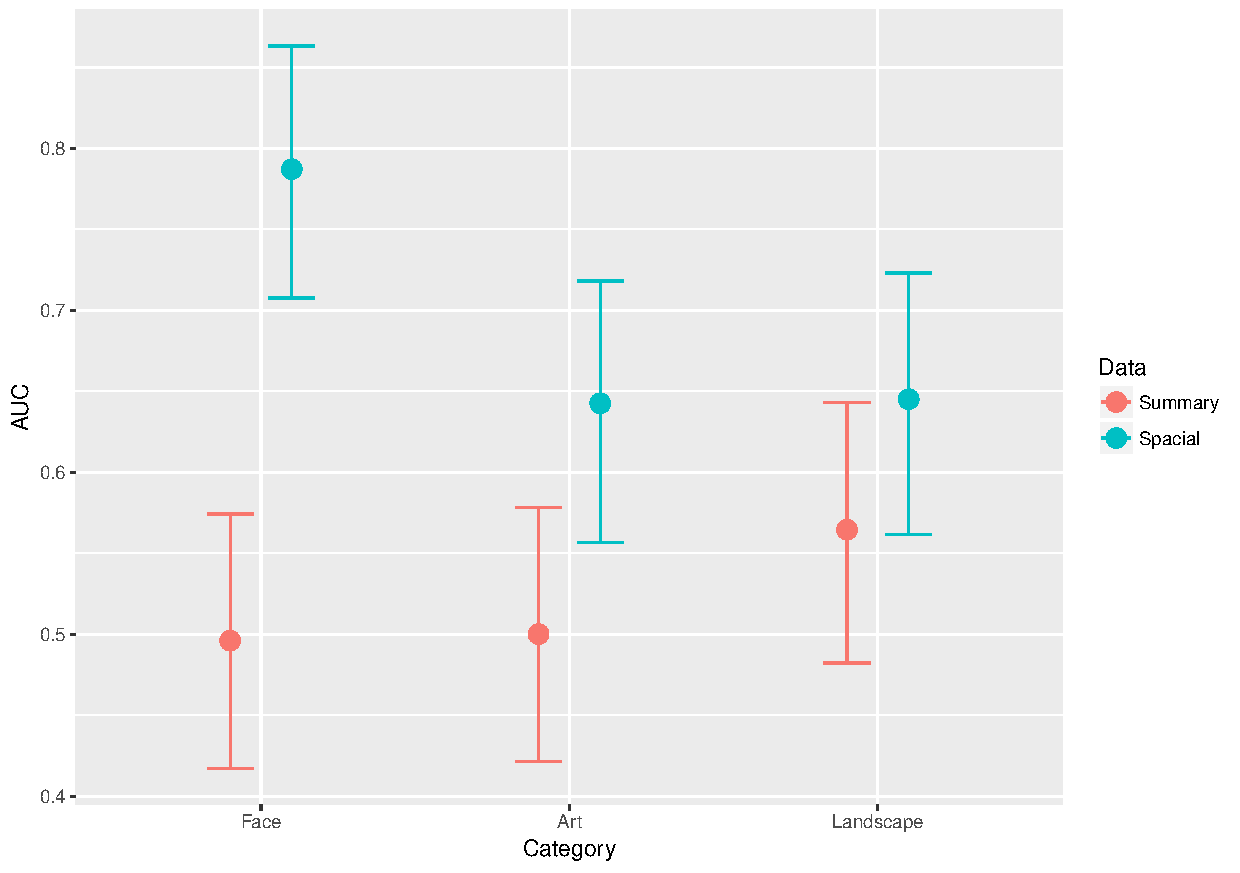
\includegraphics[width=1\textwidth]{CategoryXFeature.pdf}
\caption[Category $\times$ Features]{\label{fig:CategoryXFeature} Performance of SVM measured as area under the curve (AUC) of category $\times$ features.}
\end{figure}
\begin{figure}
\centering
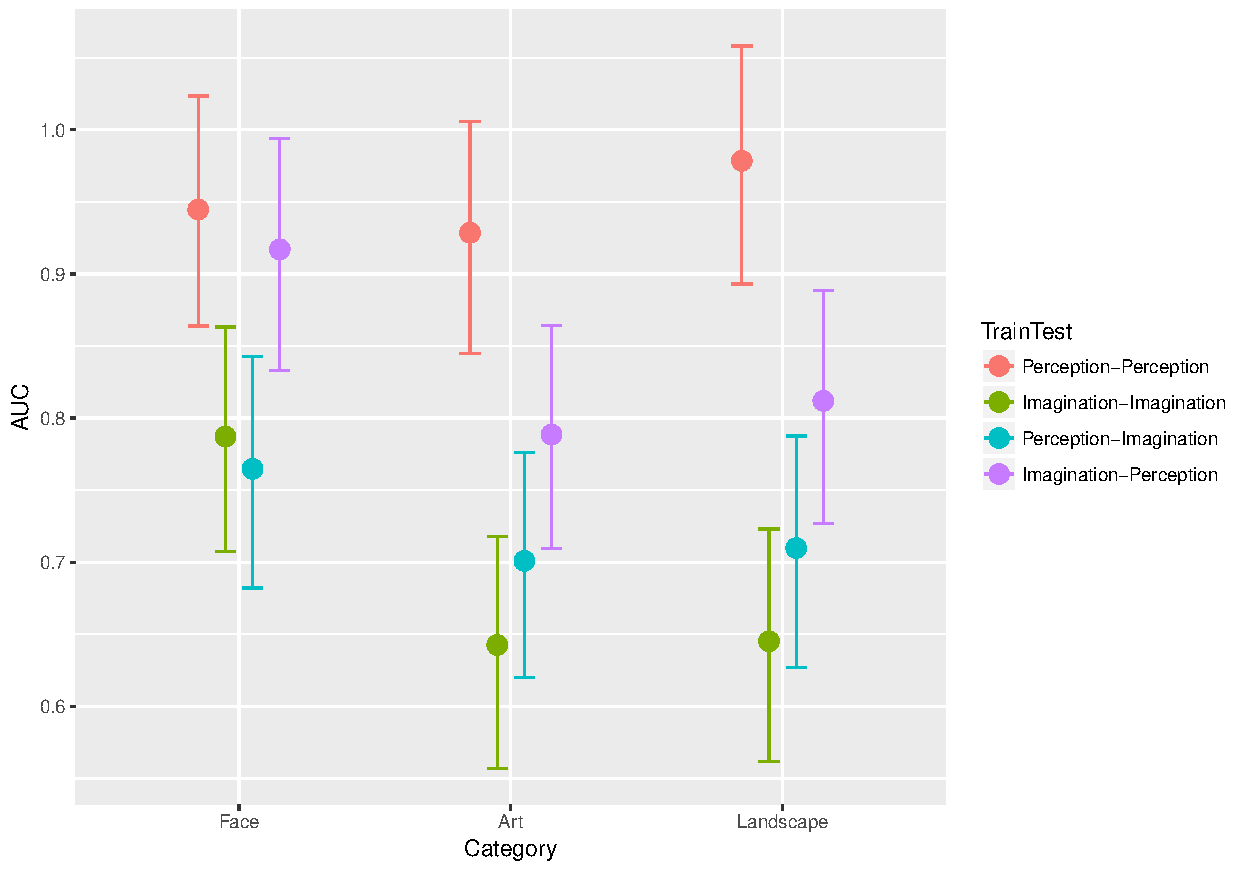
\includegraphics[width=1\textwidth]{CategoryXTrainTest.pdf}
\caption[Category $\times$ Training-Test-Condition]{\label{fig:CategoryXTrainTest} }
\end{figure}
\begin{figure}
\centering
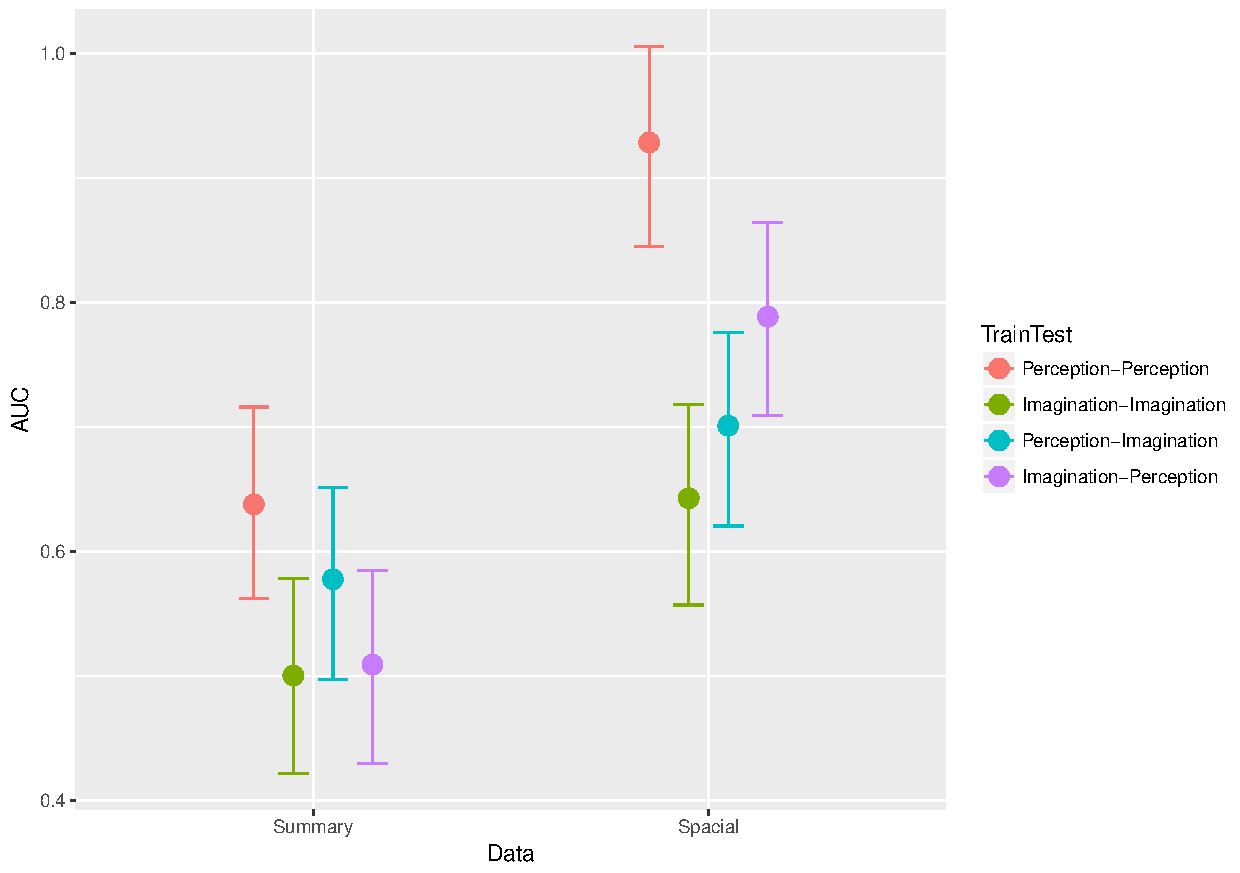
\includegraphics[width=1\textwidth]{FeatureXTrainTest.pdf}
\caption[Training-Test-Condition $\times$ Features]{\label{fig:FeatureXTrainTest} }
\end{figure}

After training the SVM the crossvalidations scores of the AUC were bootstraped and entered in to a bayesian muli level model.
That classifier performed on average above chance level, which is defined as a performance of a AUC of greater than 0.5. Both summary features and spatial features were bootstraped seperatly. Both were above chance, with the difference that spatial features ($M$ 0.81, CI[0.78;0.82]) performed better than the summary features ($M$ 0.55, CI[0.54;0.58]). \\
For the bayesian multi level model, the full model was specified as described above and backward elimination of predictors was performed. First group level effects were optimized and then population level effects were analysed. \\
Both group level effects subject ($\Delta_{LOO(full - full_{-subject})}$ -13.72 [SE 8.15]) and image ($\Delta_{LOO(full - full_{-image})}$ -54.18 [SE  14.89]) were predictors of the prediction accuracy of the SVM. On the Population the model without the three-way-interaction (f\_3WI) was superior ($\Delta_{LOO(full - full_{-f\_3WI})}$ 5.37[SE 5.33]) to the full model.  All three two-way interactions turned out texplain a relevant part of variance compared to the model without the three-wy-interaction (
Category $\times$ feature-type $\Delta_{LOO(f\_3WI - f\_3WI_{-Category \times feature\_type})}$ -60.93 [SE 16.84]; 
Category $\times$ train-test $\Delta_{LOO(f\_3WI- f\_3WI_{-Category \times train\_test})}$ -15.94 [SE  9.43];
feature-type $\times$ train-test $\Delta_{LOO(f\_3WI- f\_3WI_{- feature\_type\times train\_test})}$ -44.29[SE  13.09]).
The this final model converged with six diverging transitions. For all parameters $\hat{R}$ was smaller than 1.01, no parameter had a Monte Carlo standard error greater than 5\% of the posterior standard deviation and the effective sample size was for all parameters greater than 10\% of the total sample size.\\

In the final model, the proposed effect of better accuracy for spatial features compared to summary statistics ($\Delta$mean -0.147, CI[0.032;0.211]) was observed. 
In general the classification for art pictures and  landscapes ($\Delta$mean 0.003, CI[-0.092;0.033]) was less accurate than faces ($\Delta$mean 0.145, CI[0.047;0.176]). 
Training on imagination and testing on perception ($\Delta$mean 0.147, CI[0.084;0.168]) was classified more accurate than both training on perception ($\Delta$mean 0.059, CI[-0.003;0.079]) or imagination and crossvalidating on imagination. The posterior distribution of the AUC trained on perception and crossvalidated on perception ($\Delta$mean 0.287, CI[0.224;0.308]) was higher than any other combination fo training and testing data. \\

The two-way interaction feature-type $\times$ category given an SVM trained on imagination and tested on imagination as most conservative reference revealed an increased difference in accuracy between spatial and summary features for faces ($\Delta$mean -0.149, CI[-0.203;-0.097]) compared to art (see fig.\ref{fig:CategoryXFeature}). 
Whereas the difference between spatial and summary features was decreased for landscapes ($\Delta$mean 0.062, CI[0.027;0.114]) compared to art. 

The two-way interaction between category $\times$ training-testing-condition showed an decrease in difference of accuracy between category art to faces when trained on perception and tested with imagination ($\Delta$mean -0.081, CI[-0.156;-0.004]) or perception ($\Delta$mean -0.129, CI[-0.204;-0.054], see fig.\ref{fig:CategoryXTrainTest}). 

At last, looking at the interaction of feature-type and train-test-condition revealed an smaller increase of accuracy between summary-features and spatial-features when tested on perception and trained on imagination ($\Delta$mean -0.139, CI[-0.030;-0.079]) or on perception ($\Delta$mean -0.149, CI[-0.209;-0.088], see fig.\ref{fig:FeatureXTrainTest}).


%UPdate durch Anpassung ersetzten!
%Konfidenz intervall einführen
\newpage
\section{Discussion}
The purpose of modeling the accuracy of the AUC of the SVM was to invest if an how the spatial feature set improves the accuracy. By this approach, knowing the nature of the features and the picture categories, interpretation in how eye tracking is used during imagination and perception are possible. \\
As seen in the bootstrapping analysis the mean accuracy of the summary features is just above chance most probabal by the interaction trainig-testing-condition of perception-perception.
On the other hand we saw as expected improved AUC classification above average for spatial features in the bootstraping analysis and the bayesian multilevel model.
In the context of comparing spatial features to summary features important is the higher improvement of the AUC when tested with perception. This improvement of perception as training set could be due to the fact that there is less noise in the data since the participant was at all times confronted with the picture and due to this there was less room for any kind of lapses.
Taking the categories into consideration we saw an higher accuracy for faces, which was driven by the spatial data. Landscapes profited the least from spatial information. These two effects might be due to the properties of the the pictures. The summary of the landscapes was more informative already since the pictures had there points more distributed especially in the lower half of the picture. Since the spacial features split the pictures based on there quantils and a distribution peaking at the center of the screen can be assumed, information laying in the central part of the screen profited most from the choosen method of picture discretizing. Outer parts of the picture were summarized into bins containing more pixels, what makes them less informative. 
This interesting effect of the property of the picture category could also explain the effects of the interaction between the picture category and training-test-condition. Faces had a reduced difference in accuracy between the reference imagination and both conditions trained with perception. This could interpreted as an improvement of the classifier when trained with imagination data for both test sets. An important difference beside the fact of the picture structure discussed above could be the informative richeness of the image. It is highly plausible that an painting has more detailed information, each beeing represented as a seperate part of the image. This could cause scalings of parts of the image and alter the gaze patterns which is not expected by the current set of features. On the other hand faces are more homogenous which makes makes each bin of features more informative, since the spatial position has interpretable meaning. \\

\subsubsection{Limitationen}
There are some limitations which should be considered. Since our study was of a experimental nature only 5 participants were recorded. Eventhough we crossvalidated on subject level, our classifier might not be generalizable for other participants because of the small samplesize.
%Pictures

\subsubsection{Future perspective}
In the future it would be interessting to see whether it is possible for the imagined data to seperate the distribution of internal picture represenation and lapses. A data-driven approach which could be followed is to write an recurrent neural network trying to predict the perception data from the imagined data. As seen above, when creating features for eye tracking data the scructure of the image needs to be consideted and features need to be optimized with respect to this information. To test the assumption of scaling a window sliding approach with different scaling factors could be choosen. 
The presented spatial features choosen in this paper had the purpose of beeing in some sort similar to the commenly used summary features which could one at the time also be used in an univariate analysis. In future work advanced features could reveal more whether there is a transformation in the data between imagination and perception. An other interesting question is wether the influence of the increased level of lapses and decreased level of attention proposed in this paper could be decreased.
Further should be investigated whether the same accuracy level is achievable with more participants with less trials each. This could be beneficial for generalization aswell it could reduce the problem of repeated presentation of the same image to the same participant.
%Quellen
% integration literatur
%Selbstwert zeug und motivational usw. Interpretion sollte diskutiert werden

\begin{comment}
bla bla 
\end{comment}
\citep{Bauer2014}

\bibliographystyle{apacite} 
%http://www.ctan.org/tex-archive/biblio/bibtex/contrib/apacite/apacite.pdf 

\bibliography{/Users/mirko/Documents/bibTexLibrary/library.bib} % database is "thesis.bib" located in a "bibtex" subfolder 
\newpage
\section{Anhang}

\listoftables
\listoffigures
\clearpage
 

\begin{comment}
%%%%%%%%%%%%%%% TABLE %%%%%%%%%%%%%%%%%%             UMGEBINGT BESCHRIFTUNGEN UND ALLES PRüfen
%Deskriptiv Nebenanova
\begin{table}
\caption[Deskritivstatistik der Identifikationhypothese]{\label{tab:deskriptivNebenANOVA}Deskriptive Beschreibung der Ratings. Ergebnisse der 3 Person $\times$ 2 Messzeitpunkt $\times$ 2 Valenz der Lebensereignisse ANOVA. Gemessen wurde die erwartete Eintretenswahrscheinlichkeit des Lebensereignisses in Prozent.}
\csvreader[head to column names,
		tabular=lllrrrrr, % Add square bracket after column
		table head=\toprule \multicolumn{4}{c}{} & \multicolumn{4}{c}{Bewertung in $\%$} \\ \cmidrule{5-8}
		 \multicolumn{1}{c}{Person} & \multicolumn{1}{c}{Messzeitpunk} & \multicolumn{1}{c}{Valenz} &  \multicolumn{1}{c}{$n$} &  \multicolumn{1}{c}{M} &  \multicolumn{1}{c}{SD}&  \multicolumn{2}{c}{95\% CI }\\\midrule,
		table foot=\bottomrule,
		separator=semicolon
	]{tabellen/nebenDesk.csv}{}% 
	{\Person\ & \Messzeitpunkt & \Valence & \N & \Mean & \SD & \lo &\hi}%
	
\bigskip
\small\textit{Anmerkung}. n = Anzahl Personen, M = Mittelwert, SD = Standardabweichung, CI = Konfidenzintervall
\end{table}

%Inferenz Neben Anova
\begin{table}
\rotatebox{90}{\begin{minipage}{\textheight }
\caption[ANOVA der Identifikationshypothese]{\label{tab:inferenzNebenANOVA}Statistische Ergebnisse der 3 Person $\times$ 2 Messzeitpunkt $\times$ 2 Valenz der Lebensereignisse ANOVA. Das Alpha Niveau ist bei 0.05 angesetzt. Mauchlys Test f{\"u}r Spheriziti{\"a}t war in allen Bedingungen nicht signifikant. }
\csvreader[head to column names,
		tabular=lrrrrr *{1}{S[table-format=1.3,table-space-text-pre=<>,table-space-text-post=***]} r,
		%\multicolumn{2}{c}{Studium}\\ \cmidrule{1-2}
		table head=\toprule \multicolumn{1}{c}{Effekt} 
		& \multicolumn{1}{c}{$df_n$} 
		& \multicolumn{1}{c}{$df_d$} 
		&  \multicolumn{1}{c}{$SS_n$} 
		&  \multicolumn{1}{c}{$SS_d$} 
		&  \multicolumn{1}{c}{$F$} 
		&  \multicolumn{1}{c}{$p$} 
		& \multicolumn{1}{c}{$\eta_p^2$}\\\midrule,
		table foot=\bottomrule,
		separator=semicolon
	]{tabellen/nebenAnova.csv}{}% 
	{\Effect\ & \DFn & \DFd & \SSn & \SSd & \F & \s\p\textsuperscript{\sig} & \etap }%
	
\bigskip
\small\textit{Anmerkung}. $^{*} p\leq 0.05$. $^{**} p\leq 0.01$. $^{***} p\leq 0.001$.
\end{minipage}}
\end{table}


\begin{table}
\rotatebox{90}{\begin{minipage}{\textheight }
\caption[Post Hoc Test der Identifikationshypothese]{\label{tab:posthocNebenANOVA}Signifikante und Hypothesenrelevante Kontraste der Identifikationshypothese. Das Alpha -Niveau wurde per Tukey - Test angepasst und bei 0.05 festgelegt. } 
\begin{threeparttable}
\csvreader[head to column names,
		tabular=lrrrr *{1}{S[table-format=1.4,table-space-text-post=***]}r ,
		%\multicolumn{2}{c}{Studium}\\ \cmidrule{1-2}
		table head=\toprule \multicolumn{1}{c}{Effekt} 
		& \multicolumn{1}{c}{$\Delta$ M} 
		& \multicolumn{1}{c}{Std. Fehler } 
		&  \multicolumn{1}{c}{$df$} 
		&  \multicolumn{1}{c}{$t$} 
		&  \multicolumn{1}{c}{$p$} &\\\midrule,
		table foot=\bottomrule,
		separator=semicolon
	]{tabellen/nebenPosthoc.csv}{}% 
	{\effect\ & \estimate & \SE & \df & \t  & \p\textsuperscript{\sig}& }%
\end{threeparttable}

	\bigskip
\small\textit{Anmerkung}. $\Delta$ M = Differenz der Mittelwerte \\$^{*} p\leq 0.05$. $^{**} p\leq 0.01$. $^{***} p\leq 0.001$.
\end{minipage}}
\end{table}

%%%%%%%%%%%%%%%%%%%%Inferenz HauptAnova%%%%%%%%%%%%%%%%%%%%%%%%%%%
\begin{table}
\caption[ANOVA der Anpassungshypothese]{\label{tab:inferenzHauptANOVA}Statistische Ergebnisse der 3 Person $\times$ 2 Erw{\"u}nschtheitnschtheit $\times$ 2 Valenz der Lebensereignisse ANOVA. Das Alpha Niveau ist bei 0.05 angesetzt. Mauchlys Test f{\"u}r Spheriziti{\"a}t war in allen Bedingungen nicht signifikant. } 

\csvreader[head to column names,
		tabular=lrrrrr *{1}{S[table-format=1.3,table-space-text-post=***]} r,
		%\multicolumn{2}{c}{Studium}\\ \cmidrule{1-2}
		table head=\toprule \multicolumn{1}{c}{Effekt} 
		& \multicolumn{1}{c}{$df_n$} 
		& \multicolumn{1}{c}{$df_d$} 
		&  \multicolumn{1}{c}{$SS_n$} 
		&  \multicolumn{1}{c}{$SS_d$} 
		&  \multicolumn{1}{c}{$F$} 
		&  \multicolumn{1}{c}{$p$} 
		& \multicolumn{1}{c}{$\eta_p^2$}\\\midrule,
		table foot=\bottomrule,
		separator=semicolon
	]{tabellen/hauptAnova.csv}{}% 
	{\Effect\ & \DFn & \DFd & \SSn & \SSd & \F & \p\textsuperscript{\sig}  & \etap}%
	

	\bigskip
\small\textit{Anmerkung}. $^{*} p\leq 0.05$. $^{**} p\leq 0.01$. $^{***} p\leq 0.001$.
\end{table}

%%%%%%%%%%%%%%%%%%%%% LMM 

\begin{table}
\caption[Deskritivstatistik der Anpassungshypothese]{\label{tab:deskLMM_all} Deskriptive Beschreibung der Anpassung der Eintretenswahrscheinlichkeit geordnet nach Faktoren der Person, des Erw\"unschtheitund der Valenz kontrolliert f\"ur Sch\"atzfehler f\"ur das gesamte Modell.}
\csvreader[head to column names,
		tabular=lllrrrrr, % Add square bracket after column
		table head=\toprule \multicolumn{4}{c}{} & \multicolumn{4}{c}{Anpassung} \\ \cmidrule{5-8}
		 \multicolumn{1}{c}{Person} 
		 & \multicolumn{1}{c}{Messzeitpunk} 
		 & \multicolumn{1}{c}{Valenz} 
		 &  \multicolumn{1}{c}{$df$} 
		 &  \multicolumn{1}{c}{M} 
		 &  \multicolumn{1}{c}{SE}
		 &  \multicolumn{2}{c}{95\% CI }\\\midrule,
		table foot=\bottomrule,
		separator=semicolon
	]{tabellen/lmmDesk.csv}{}% 
	{\Person\ & \desirable & \Valence & \df & \lsmean & \SE & \lo &\hi}%
	
\bigskip
\small\textit{Anmerkung}. df = Freiheitsgrade , M = Mittelwert, SE = Standardfehler, CI = Konfidenzintervall
\end{table}

\begin{table}
\rotatebox{90}{\begin{minipage}{\textheight}
\caption[Gesammtes lineare gemischte Modell der Anpassungshypothese]{\label{tab:LMM_Model_all} Gesamtes lineares gemischtes Modell mit Person, Valenz, Erw\"unschtheit als fixierter Faktor, Sch\"atzfehler als Kovarianz und Versuchsperson als Zufallsfaktor.} 

\begin{threeparttable}
\csvreader[head to column names,
		tabular=lrrrr *{1}{S[table-format=1.3,table-space-text-post=***]}r ,
		%\multicolumn{2}{c}{Studium}\\ \cmidrule{1-2}
		table head=\toprule \multicolumn{1}{c}{Effekt} 
		& \multicolumn{1}{c}{$b$ } 
		& \multicolumn{1}{c}{SE} 
		&  \multicolumn{1}{c}{$df$} 
		&  \multicolumn{1}{c}{$t$} 
		&  \multicolumn{1}{c}{$p$} &\\\midrule,
		table foot=\bottomrule,
		separator=semicolon
	]{tabellen/lmmModel.csv}{}% 
	{\Effect\ & \b & \StdError & \DF & \Tvalue & \Pvalue\textsuperscript{\sig}& }%
	
\end{threeparttable}

	\bigskip
\small\textit{Anmerkung}. PE = Positives Ereignis $^{*} p\leq 0.05$. $^{**} p\leq 0.01$. $^{***} p\leq 0.001$.
\end{minipage}}
\end{table}


%%%%%%%%%%%%%%%%%% LMM SUB
\begin{table}
\caption[Deskriptivstatistik der Anpassungshypothese nach Valenz]{\label{tab:deskLMM_PN} Deskriptive Beschreibung der Anpassung der Eintretenswahrscheinlichkeit unterteilt in ein Untermodell f\"ur positive Lebensereignisse und eines f\"ur negative Lebensereignisse. Beide unterteilt nach Person und Er\"unschtheit, sowie kontrolliert f\"ur den Sch\"atzfehler.}
\csvreader[head to column names,
		tabular=llllrrrrr, % Add square bracket after column
		table head=\toprule \\\multicolumn{5}{c}{ } & \multicolumn{3}{c}{Anpassung} \\ \cmidrule{6-8}
		 \multicolumn{1}{c}{Modell} 
		 & \multicolumn{1}{c}{Person} 
		 & \multicolumn{1}{c}{Messzeitpunk} 
		 &  \multicolumn{1}{c}{$df$} 
		 &  \multicolumn{1}{c}{M} 
		 &  \multicolumn{1}{c}{SE}
		 &  \multicolumn{2}{c}{95\% CI }\\\midrule,
		table foot=\bottomrule,
		separator=semicolon
	]{tabellen/lmmPNDesk.csv}{}% 
	{\Modell & \Person\ & \desirable & \df & \lsmean & \SE & \lo &\hi }%
	
\bigskip
\small\textit{Anmerkung}. df = Freiheitsgrade , M = Mittelwert, SE = Standardfehler, CI = Konfidenzintervall.

\end{table}

\begin{table}
\rotatebox{90}{\begin{minipage}{\textheight}
\caption[Linear gemischtes Modell der Anpassungshypothese nach Valenz]{\label{tab:LMM_Model_PN} Lineares gemischtes Modell f\"ur je positive und negative Ereignisse mit Person und Erw\"unschtheit als fixierten Faktor, Sch\"atzfehler als Kovarianz und Versuchsperson als Zufallsfaktor.} 

\begin{threeparttable}
\csvreader[head to column names,
		tabular=llrrrr *{1}{S[table-format=1.3,table-space-text-post=***]}r ,
		%\multicolumn{2}{c}{Studium}\\ \cmidrule{1-2}
		table head=\toprule \multicolumn{1}{c}{Modell} 
		& \multicolumn{1}{c}{Effekt} 
		& \multicolumn{1}{c}{$b$ } 
		& \multicolumn{1}{c}{SE} 
		&  \multicolumn{1}{c}{$df$} 
		&  \multicolumn{1}{c}{$t$} 
		&  \multicolumn{1}{c}{$p$} &\\\midrule,
		table foot=\bottomrule,
		separator=semicolon
	]{tabellen/lmmPNModel.csv}{}% 
	{\Modell &\Effect\ & \b & \StdError & \DF & \Tvalue & \Pvalue\textsuperscript{\sig}& }%
	
\end{threeparttable}

	\bigskip
\small\textit{Anmerkung}. $^{*} p\leq 0.05$. $^{**} p\leq 0.01$. $^{***} p\leq 0.001$.
\end{minipage}}
\end{table}

%%%%%%%%%%% posthoc LMM

\begin{table}
\rotatebox{90}{\begin{minipage}{\textheight }
\caption[Post Hoc Test der Anpassungshypothese positiver Items]{\label{tab:LMM_posthoc_P} Hypothesenrelevante Kontraste f\"ur das linear gemischte Modell f\"ur positive Ereignisse. Das Alpha -Niveau wurde per Tukey - Test angepasst und bei 0.05 festgelegt.} 
\begin{threeparttable}
\csvreader[head to column names,
		tabular=lrrrr *{1}{S[table-format=1.3,table-space-text-post=***]}r ,
		%\multicolumn{2}{c}{Studium}\\ \cmidrule{1-2}
		table head=\toprule \multicolumn{1}{c}{Effekt} 
		& \multicolumn{1}{c}{$\Delta$ M} 
		& \multicolumn{1}{c}{SE} 
		&  \multicolumn{1}{c}{$df$} 		
		&  \multicolumn{1}{c}{$t$} 
		&  \multicolumn{1}{c}{$p$} &\\\midrule,
		table foot=\bottomrule,
		separator=semicolon
	]{tabellen/lmmPosthocP.csv}{}% 
	{\effect\ & \estimate & \SE & \df & \t  & \p\textsuperscript{\sig}& }%
\end{threeparttable}

	\bigskip
\small\textit{Anmerkung}. $\Delta$ M = Differenz der Mittelwerte \\$^{*} p\leq 0.05$. $^{**} p\leq 0.01$. $^{***} p\leq 0.001$.
\end{minipage}}
\end{table}

\begin{table}
\rotatebox{90}{\begin{minipage}{\textheight }
\caption[Post Hoc Test der Anpassungshypothese negativer Items]{\label{tab:LMM_posthoc_N} Hypothesenrelevante Kontraste f\"ur das linear gemischte Modell f\"ar negative Ereignisse. Das Alpha -Niveau wurde per Tukey - Test angepasst und bei 0.05 festgelegt.} 
\begin{threeparttable}
\csvreader[head to column names,
		tabular=lrrrr *{1}{S[table-format=1.3,table-space-text-post=***]}r ,
		%\multicolumn{2}{c}{Studium}\\ \cmidrule{1-2}
		table head=\toprule \multicolumn{1}{c}{Effekt} 
		& \multicolumn{1}{c}{$\Delta$ M} 
		& \multicolumn{1}{c}{SE } 
		&  \multicolumn{1}{c}{$df$} 		
		&  \multicolumn{1}{c}{$t$} 
		&  \multicolumn{1}{c}{$p$} &\\\midrule,
		table foot=\bottomrule,
		separator=semicolon
	]{tabellen/lmmPosthocN.csv}{}% 
	{\effect\ & \estimate & \SE & \df & \t  & \p\textsuperscript{\sig}& }%
\end{threeparttable}

\bigskip
\small\textit{Anmerkung}. $\Delta$ M = Differenz der Mittelwerte \\$^{*} p\leq 0.05$. $^{**} p\leq 0.01$. $^{***} p\leq 0.001$.
\end{minipage}}
\end{table}

\begin{comment}


%LEBENSEREIGNISSE
\begin{table}
\caption{\label{tab:LMM_posthoc_N} Auflistung der benutzten Lebensereignisse mit der jeweiligen Zuteilung zum Zeitraum, der Valenz, der R\"uckmeldung und der Gruppe.} 
\begin{threeparttable}
\csvreader[head to column names,
		tabular=lrrrrr ,
		%\multicolumn{2}{c}{Studium}\\ \cmidrule{1-2}
		table head=\toprule 
		 \multicolumn{1}{c}{Lebensereignisse} 
		& \multicolumn{1}{c}{Zeitraum } 
		&  \multicolumn{1}{c}{Valenz} 		
		&  \multicolumn{1}{c}{R\"uckmeldung} 
		&  \multicolumn{1}{c}{Gruppe} &\\\midrule,
		table foot=\bottomrule,
		separator=semicolon
	]{tabellen/Lebensereignisse.csv}{}% 
	{\Lebensereignis & \Zeitraum & \Valenz & \Ruckmeldung & \Gruppe }%
\end{threeparttable}

%\bigskip
%\small\textit{Anmerkung}. $\Delta$ M = Differenz der Mittelwerte \\$^{*} p\leq 0.05$. $^{**} p\leq 0.01$. $^{***} p\leq 0.001$.

\end{table}
\end{comment}





\end{document}

%
% Please see the package documentation for more information
% on the APA6 document class:
%
% http://www.ctan.org/pkg/apa6
%
